\label{ch:methodology}
\section{Research Design and Narrative Overview}
\label{sec:method-design}

This thesis follows a \textbf{design--implement--evaluate} methodology. Chapter~\ref{ch:eda} established what the Multi-LexSum corpus looks like in practice and which modelling assumptions are unsafe (complete short/tiny coverage; full-document encoding). The present chapter translates those findings into an implemented dual-system pipeline, in the sense used throughout this thesis: a fast, pattern-matching neural component (\textbf{System~1}) that drafts fluent text without any guarantee that its claims are checkable, paired with a slower, rule-governed component (\textbf{System~2}) that audits a specific, well-defined class of those claims, case citations, against an external source of truth. The terminology follows Kahneman's dual-process account of fast, associative versus slow, deliberative reasoning \cite{kahneman2011thinkingbook}, as adapted to system design by neuro-symbolic AI arguments that System~1 (neural) outputs need System~2 (symbolic, deliberative) checks in domains where an unchecked error carries professional or safety consequences \cite{kautz2022thirdaisummer}. Concretely, System~1 is Module~A (Section~\ref{sec:module-a}); System~2 is Modules~B and~C plus the bounded correction policy (Sections~\ref{sec:module-b}--\ref{sec:correction}).

The design is deliberately \emph{asymmetric}. Neural models remain responsible for fluent multi-document abstraction, a task where they excel \cite{xiao2022primera,shen2022multilexsum}. They are \emph{not} trusted as the final authority on whether a case citation exists. That authority is delegated to an auditable symbolic layer backed by CourtListener \cite{courtlistener_api,eyecite2021}, consistent with the System~1/System~2 division above: System~1 is never asked to self-certify a claim it has no mechanism to verify.

\begin{enumerate}
  \item \textbf{Baseline generation.} Produce long ($D\rightarrow L$) draft summaries with PRIMERA under an explicit truncation budget motivated by Chapter~\ref{ch:eda}.
  \item \textbf{Citation extraction and verification.} Extract \texttt{FullCaseCitation} spans with eyecite; verify each span against CourtListener; assign Verified / Mismatch / Ambiguous / NotFound / Malformed labels.
  \item \textbf{Bounded correction.} Redact unverifiable cites; safely repair soft mismatches; leave or \emph{re-anchor} Ambiguous cites; never substitute a contradicting CourtListener case name.
  \item \textbf{Paired evaluation.} Track each draft citation through correction using stable \texttt{citation\_id}s; report paired hallucination rate (HR) jointly with ROUGE-L.
\end{enumerate}

A preliminary citation-rich validation subset ($n=10$) is used during development to stress-test labelling and correction policies. Those numbers are reported as \textbf{pilot evidence} only; they do not replace a full validation/test evaluation in later chapters.

\section{End-to-End Architecture}
\label{sec:method-architecture}

Figure~\ref{fig:architecture} shows the implemented pipeline. Relative to earlier design sketches that assumed free-form LLM regeneration of the entire summary, the correction stage is now primarily \textbf{symbolic} (span redact / replace / re-anchor), with an optional light LLM rewrite path that must re-verify.

\begin{figure}[!t]
\centering
\begin{tikzpicture}[
  font=\small,
  node distance=9mm and 7mm,
  box/.style={draw, rounded corners, align=center, inner sep=5pt, text width=2.35cm},
  arrow/.style={-Latex, thick}
]
\node[box] (input) {Multi-LexSum\\sources\\(truncated)};
\node[box, right=of input] (summ) {Module A\\PRIMERA\\draft $s_0$};
\node[box, right=of summ] (extract) {Module B\\eyecite\\full spans};
\node[box, right=of extract] (verify) {Module C\\CourtListener\\labels};
\node[box, right=of verify] (corr) {Correction\\redact / repair\\/ re-anchor};
\node[box, below=12mm of corr] (eval) {Paired HR + ROUGE-L\\(+ optional McNemar)};

\draw[arrow] (input) -- (summ);
\draw[arrow] (summ) -- (extract);
\draw[arrow] (extract) -- (verify);
\draw[arrow] (verify) -- (corr);
\draw[arrow] (corr) -- (eval);
\draw[arrow] (verify) -- node[left, align=right, font=\scriptsize]{Ambiguous\\/ unsafe} ++(0,-6mm) -| (corr);
\end{tikzpicture}
\caption{Dual-system architecture as implemented: neural draft generation followed by symbolic citation verification and bounded correction. Evaluation tracks draft citations through correction (paired HR).}
\label{fig:architecture}
\end{figure}

\section{Module A: Neural Summarization}
\label{sec:module-a}

\subsection{Why PRIMERA}
Module~A uses PRIMERA \cite{xiao2022primera}, a multi-document summarization model that is a strong Multi-LexSum baseline \cite{shen2022multilexsum}. The choice is pragmatic and scientific: (i)~it matches the benchmark setting against which ROUGE improvements are usually claimed; (ii)~it forces the thesis to confront citation faithfulness on a realistic neural draft rather than on toy extractive baselines.

\subsection{Why $D\rightarrow L$ only}
Chapter~\ref{ch:eda} showed that long summaries are complete for every case, while short and tiny fields are systematically missing, and that heuristic citation density is highest in long targets. Primary experiments therefore use document-to-long ($D\rightarrow L$) summarization. Short/tiny settings remain available for future ablation, not for the core RQ answers.

\subsection{Truncation policy}
EDA demonstrated that more than 90\% of training cases exceed an 8{,}192-token budget and that even 131k-token budgets leave a non-trivial residue. Module~A therefore applies an explicit \textbf{naive truncation} to a fixed token budget (4{,}096 tokens, the architectural ceiling of the PRIMERA checkpoint used for the full-scale run, confirmed from its \texttt{max\_encoder\_position\_embeddings}, not a demo-time simplification). This is an honest operating constraint, not a claim of optimal long-context modelling. The dual-system thesis \emph{depends} on this honesty: if the model cannot see the full docket, symbolic verification of citations becomes more important, not less \cite{maynez2020faithfulness,beltagy2020longformer}.

\subsection{Generation length calibration}
Full-scale generation initially produced summaries well short of the $D\rightarrow L$ target (mean 461 words against an $\approx$850-token/650-word budget). Inspection traced this to the PRIMERA checkpoint's own \texttt{generation\_config.json}, which ships \texttt{length\_penalty=0}: with no length normalization, beam search scores candidates by raw summed log-probability, which mathematically favours shorter sequences, since every additional token multiplies in a probability $\le 1$. Nothing in the pipeline overrode this default. Module~A now sets an explicit \texttt{min\_new\_tokens} floor and \texttt{length\_penalty=2.0}, raising mean length to 535 words. This is reported as a calibration decision, not a result: it establishes that the citation-attempt comparisons across generators in Section~\ref{sec:module-a-crossmodel} reflect genuine generation behaviour rather than an unexamined default.

Listing~\ref{lst:module-a-generate} shows the calibrated call as implemented: the explicit \texttt{min\_new\_tokens} and \texttt{length\_penalty} arguments are the fix, not defaults inherited from the checkpoint.

\begin{lstlisting}[caption={Module~A batch generation call with the length-calibration fix explicit (\href{\repourl/blob/main/src/module_a_summarizer/generate.py}{\texttt{src/module\_a\_summarizer/generate.py}}).}, label={lst:module-a-generate}]
max_new_tokens = config["max_new_tokens"][granularity]
min_new_tokens = config.get("min_new_tokens", {}).get(granularity)
length_penalty = config.get("length_penalty", 2.0)  # overrides checkpoint's 0
num_beams = config.get("num_beams", 5)

for case in pending:
    generated = summarizer.generate(
        case.sources_text,
        max_new_tokens=max_new_tokens,
        num_beams=num_beams,
        min_new_tokens=min_new_tokens,
        length_penalty=length_penalty,
        early_stopping=early_stopping,
    )
    _append_row(out_path, {"case_id": case.case_id, "generated_summary": generated, ...})
\end{lstlisting}

\subsection{Cross-model comparison: LLM and LLM+retrieval variants}
\label{sec:module-a-crossmodel}

Development-time inspection of full-scale PRIMERA drafts showed markedly fewer attempted case citations than the corresponding expert summaries on the same citation-dense cases, an observation that motivates, rather than answers, a question this thesis is positioned to test: is low citation-attempt density a property of neural legal summarization in general, or an artefact of one checkpoint's output-length ceiling and truncation window? To probe this, Module~A is extended with two further generators evaluated on the identical case set:

\begin{itemize}
  \item \textbf{LLM zero-shot.} Qwen2.5-7B-Instruct \cite{qwen2025qwen25,yang2024qwen2}, an instruction-tuned open-weight model (Apache-2.0), given an 8{,}192-token input budget (double PRIMERA's architecturally fixed 4{,}096 above) and an explicit instruction to preserve every real case citation present in the source material, with an approximately 2{,}000-token output budget.
  \item \textbf{LLM + retrieval.} The same checkpoint and budgets, but source documents are ranked by a fast citation-density heuristic before truncation, rather than kept in naive chronological order. Ranking uses a regex proxy for citation-like patterns rather than a full eyecite parse: eyecite's cross-reference resolution over the full, untruncated source text of 100 dockets (some exceeding 100{,}000 tokens each) is not fast enough to justify for what is only a coarse relevance signal, and precise extraction downstream (Module~B) is unaffected by this choice. This variant operationalizes, for the first time inside this pipeline rather than by citation to prior work, the retrieval-versus-symbolic-verification distinction the literature review raises (Section~\ref{sec:lit-rag}, Table~\ref{tab:rag-vs-symbolic}).
\end{itemize}

Both variants are evaluated under the same generate--verify--correct pipeline (Sections~\ref{sec:module-b}--\ref{sec:correction}) and the same four conditions (Section~\ref{sec:conditions}) as the PRIMERA baseline, producing a $3\times4$ generator--condition matrix. Comparative citation-attempt counts, hallucination rates, and quality metrics across the three generators are reported in the results chapter once full-scale verification of all three completes.

\section{Module B: Case Citation Extraction}
\label{sec:module-b}

Module~B uses eyecite \cite{eyecite2021} to extract \texttt{FullCaseCitation} objects from draft text. Three implementation details are central to evaluation integrity:

\begin{itemize}
  \item \textbf{Full spans.} Replacements operate on the full citation span (including party names when present), not only the reporter substring. Reporter-only edits historically produced garbled hybrids (case name spliced into a reporter fragment).
  \item \textbf{Stable \texttt{citation\_id}.} Each extracted citation receives an identifier derived from normalized cite text and character offsets, enabling paired tracking from draft to corrected summary.
  \item \textbf{Markup sanitization.} Multi-LexSum source documents retain HTML markup from their originating court-record/Clearinghouse pages (e.g.\ \texttt{<i>Obergefell v.\ Hodges</i>}), which extractive-leaning PRIMERA drafts can copy verbatim; LLM-generated drafts introduce analogous Markdown emphasis (\texttt{**Graham**}). Either corrupts eyecite's antecedent/party-name guessing when markup sits directly adjacent to a case name, observed directly in development runs and traced to malformed \texttt{party\_names} extraction (e.g.\ \texttt{("", "Hodges</i>")} instead of \texttt{("Obergefell", "Hodges")}) that propagated into an incorrect correction-loop outcome for an otherwise real, correctly identifiable citation. Extraction now blanks HTML tags and Markdown emphasis markers with equal-length whitespace before parsing, length-preserving, so citation-span character offsets used elsewhere for redaction and replacement remain valid against the original text.
\end{itemize}

Listing~\ref{lst:module-b-blank} shows the markup-blanking fix: tags and Markdown emphasis are replaced with equal-length whitespace, not deleted, so every downstream character offset used for redaction or replacement still lines up with the original text.

\begin{lstlisting}[caption={Length-preserving markup blanking before eyecite parsing (\href{\repourl/blob/main/src/module_b_extraction/extract_citations.py}{\texttt{src/module\_b\_extraction/extract\_citations.py}}).}, label={lst:module-b-blank}]
_MARKUP_RE = re.compile(r"</?i>|</?b>|</?em>|</?strong>|\*\*|<a\s[^>]*>|</a>")

def _blank_markup(text: str) -> str:
    return _MARKUP_RE.sub(lambda m: " " * len(m.group()), text)

def extract_citations(summary_text: str) -> list[ExtractedCitation]:
    cleaned_text = _blank_markup(summary_text)
    results = []
    for c in get_citations(cleaned_text):
        if not isinstance(c, FullCaseCitation):
            continue
        results.append(ExtractedCitation(
            raw_text=c.corrected_citation_full(),
            normalized=str(c.corrected_citation()),
            party_names=_party_names_from_citation(c),
            span=_full_span_from_citation(c),
            citation_id=make_citation_id(...),
        ))
    return results
\end{lstlisting}

Extraction is deliberately narrower than ``any legal reference'': pin cites and some proprietary identifiers are handled as attributes of a full case citation when eyecite exposes them. This reduces false positives in hallucination accounting at the cost of missing some informal references, a trade-off stated explicitly for RQ1.

\section{Module C: Symbolic Verification}
\label{sec:module-c}

Module~C queries CourtListener's citation lookup API \cite{courtlistener_api} and assigns one of five labels. Table~\ref{tab:label-taxonomy} is the canonical glossary used throughout the thesis.

\begin{table}[!t]
\centering
\caption{CourtListener verification label taxonomy (Module~C).}
\label{tab:label-taxonomy}
\begin{tabular}{@{}p{2.3cm}p{5.2cm}p{5.0cm}@{}}
\toprule
\textbf{Label} & \textbf{Meaning} & \textbf{Default correction action} \\
\midrule
Verified & Status 200 and parties/year compatible with the matched cluster & Keep \\
Mismatch & Resolves, but metadata incompletely matches \emph{without} hard party contradiction & Safe CL-name repair when identity is compatible \\
Ambiguous & Status 300 (multi-cluster) \emph{or} hard party contradiction with the resolved cluster & Leave highlighted; re-anchor if a Verified same-case cite exists \\
NotFound & Status 404 & Redact \\
Malformed & Status 400 / unparseable & Redact \\
\bottomrule
\end{tabular}
\end{table}

Listing~\ref{lst:module-c-label} is the code that implements Table~\ref{tab:label-taxonomy} directly: each CourtListener response status maps to exactly one label, and the Verified/Ambiguous split within a status-200 response is decided by \texttt{fields\_match} and the hard-party-contradiction check described below.

\begin{lstlisting}[caption={CourtListener status to taxonomy-label mapping (\href{\repourl/blob/main/src/module_c_verifier/verify.py}{\texttt{src/module\_c\_verifier/verify.py}}).}, label={lst:module-c-label}]
def _label_from_status(status, extracted, cluster, *, fuzzy_threshold):
    if status == 404:
        return "NotFound", "No matching citation in CourtListener's database.", None, None
    if status == 300:
        return "Ambiguous", "Citation matches multiple case clusters.", None, None
    if status == 400:
        return "Malformed", "Citation could not be parsed as a valid reporter.", None, None
    if status == 200 and cluster:
        case_name = cluster.get("case_name")
        if fields_match(extracted, cluster, fuzzy_threshold=fuzzy_threshold):
            return "Verified", "Citation and metadata both confirmed.", case_name, cluster.get("date_filed")
        # Hard party contradiction: wrong CL cluster identity -- leave Ambiguous.
        if case_name and _party_names_contradict(extracted, case_name):
            return "Ambiguous", f"Parties contradict draft case name ({case_name}).", case_name, None
        return "Mismatch", f"Resolves, but metadata does not match cluster ({case_name}).", case_name, None
    return "Malformed", "Unexpected CourtListener response.", None, None
\end{lstlisting}

\subsection{Why Ambiguous is not ``Mismatch repair''}
Early prototypes treated every metadata disagreement as a Mismatch and replaced the draft span with CourtListener's \texttt{case\_name}. That policy is unsafe when the reporter/LEXIS string resolves to the \emph{wrong matter}: a Brown desegregation draft can be rewritten to an unrelated commercial case that happens to share a proprietary identifier. The implemented policy therefore promotes hard party contradictions to \textbf{Ambiguous} and forbids substituting the contradicting cluster name.

A related refinement applies once a repair is judged safe: the corrected citation string now always prefers CourtListener's verified \texttt{date\_filed} over the draft's own year, not only when the draft supplied no year at all. Mismatches are frequently exactly a year discrepancy on an otherwise correctly identified citation (e.g.\ a real Supreme Court case with a hallucinated decision year); keeping the draft's wrong year in a ``repaired'' citation left it failing re-verification on every subsequent correction iteration, exhausting the iteration budget on a case that should have resolved on the first pass.

\subsection{Why CourtListener}
CourtListener provides an open, reproducible legal API operated by the Free Law Project \cite{freelawproject}, enabling auditable per-citation explanations rather than closed commercial ``hallucination-free'' claims \cite{magesh2025hallucinationfree}. Rate limits and caching are first-class engineering constraints in the implementation: the account's confirmed access level (10 requests/minute, 100/hour, 250/day) is enforced by a persistent, three-tier local rate limiter alongside a SQLite response cache, so verification runs can pause and resume across process restarts and multi-day full-scale runs without exceeding the API's real limits.

Figure~\ref{fig:courtlistener-api-usage} shows this account's own Developer Tools dashboard: the confirmed 10/100/250 access level and, at the time of the full-scale run, 565 API requests made all-time, consistent with a multi-day verification schedule paced by the daily cap rather than a single burst of calls.

\begin{figure}[!t]
\centering
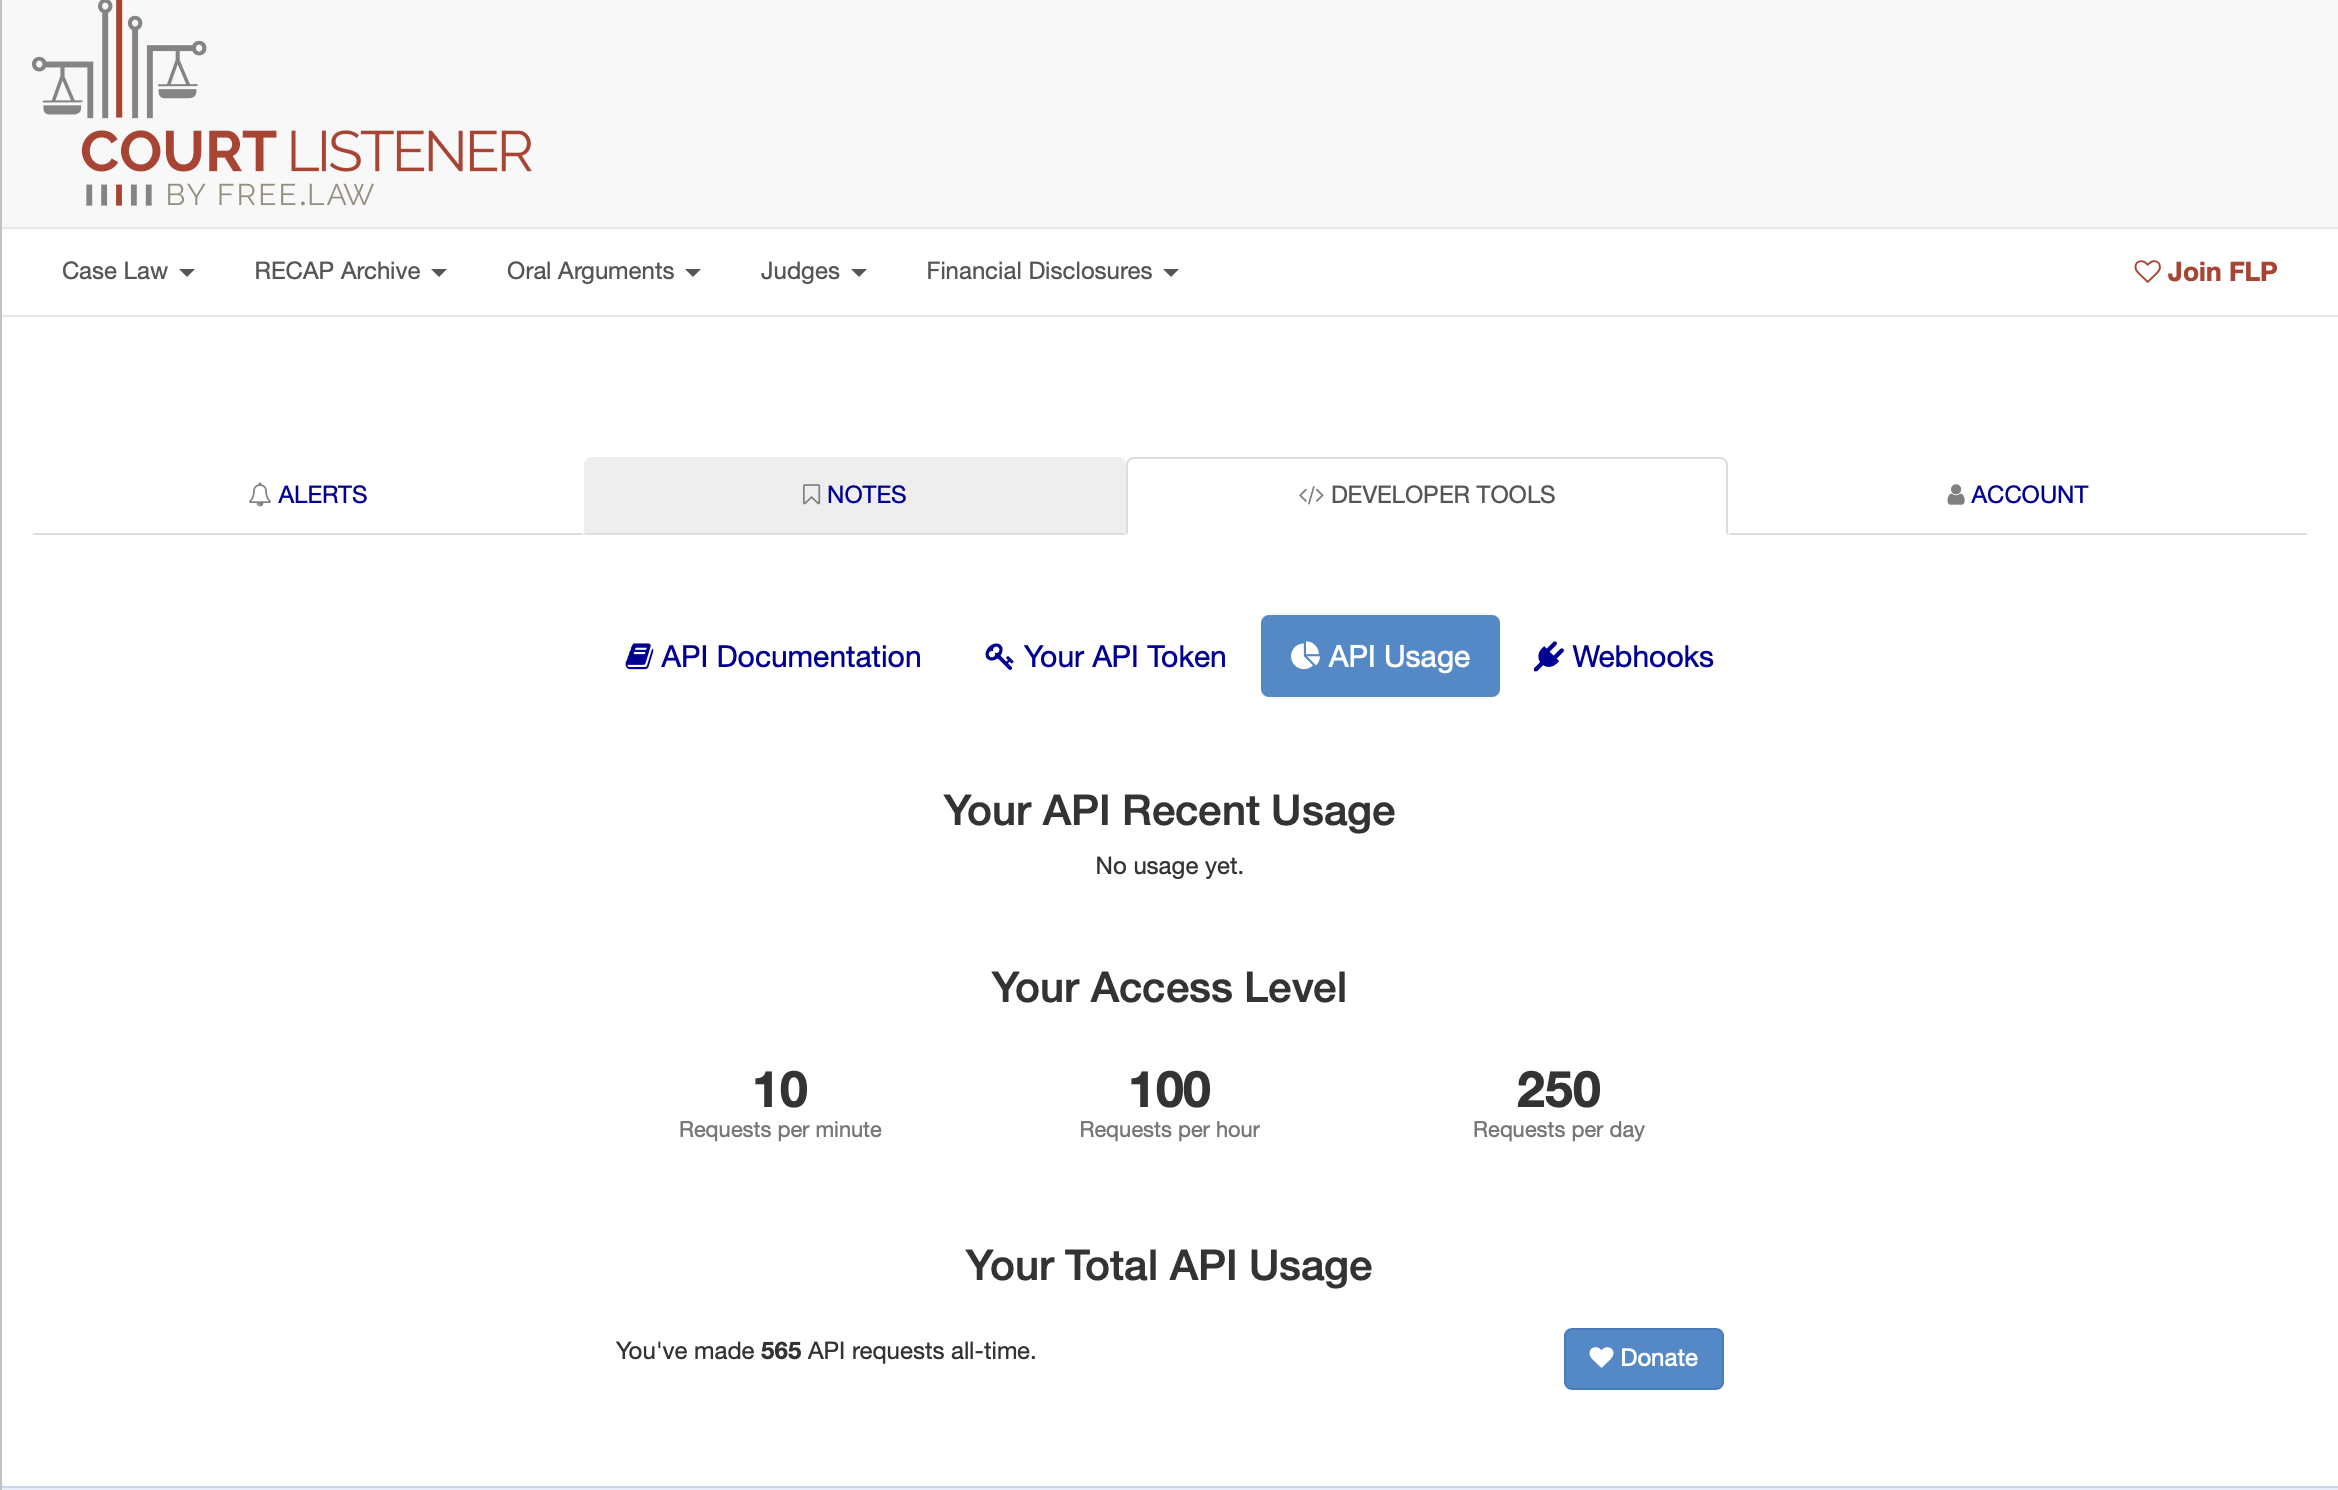
\includegraphics[width=0.85\linewidth]{courtlistener_api_usage.png}
\caption{CourtListener Developer Tools: confirmed API access level (10/min, 100/hour, 250/day) and cumulative request count for the account used in this thesis.}
\label{fig:courtlistener-api-usage}
\end{figure}

\section{Bounded Symbolic Correction}
\label{sec:correction}

Figure~\ref{fig:workflow} summarizes the runtime workflow for one case.

\begin{figure}[!t]
\centering
\begin{tikzpicture}[
  font=\small,
  node distance=7mm,
  workflowstep/.style={draw, rectangle, rounded corners, align=left, inner sep=5pt, text width=0.92\linewidth},
  arrow/.style={-Latex, thick}
]
\node[workflowstep] (s1) {1) Generate draft summary $s_0$ (Module~A / PRIMERA)};
\node[workflowstep, below=of s1] (s2) {2) Extract full-span citations $C_{s_0}$ (Module~B / eyecite)};
\node[workflowstep, below=of s2] (s3) {3) Verify each $c\in C_{s_0}$ via CourtListener (Module~C)};
\node[workflowstep, below=of s3] (s4) {4) Correct: redact NotFound/Malformed; repair safe Mismatch; re-anchor Ambiguous when a Verified same-case cite exists; otherwise leave Ambiguous};
\node[workflowstep, below=of s4] (s5) {5) Re-verify; emit final summary + paired outcomes (max $K$ iterations)};

\draw[arrow] (s1) -- (s2);
\draw[arrow] (s2) -- (s3);
\draw[arrow] (s3) -- (s4);
\draw[arrow] (s4) -- (s5);
\end{tikzpicture}
\caption{Generate--verify--correct workflow as implemented (symbolic correction with optional re-anchor).}
\label{fig:workflow}
\end{figure}

\subsection{Re-anchor policy}
When an Ambiguous or unsafe citation has draft parties compatible with a \textbf{Verified} citation elsewhere in the same summary, the system replaces the bad span with the verified citation string (``re-anchor''). This recovers cases such as a wrong LEXIS identifier attached to an otherwise correct Brown party string when \texttt{98 F.\ Supp.\ 797} already verified in-summary. If no anchor exists, the Ambiguous cite remains in text and counts toward paired HR as \texttt{still\_bad}.

\subsection{Formal correction policy}
\label{sec:correction-formal}
Table~\ref{tab:label-taxonomy} and Figure~\ref{fig:workflow} are equivalent to the following decision rule, stated once here to make the policy checkable independent of its prose description. Let $\ell(c) \in \{\texttt{Verified}, \texttt{Mismatch}, \texttt{Ambiguous}, \texttt{NotFound}, \texttt{Malformed}\}$ be Module~C's label for draft citation $c$, and let $\mathrm{anchor}(c) \in \{\texttt{true}, \texttt{false}\}$ indicate whether a party-compatible \texttt{Verified} citation exists elsewhere in the same draft. The correction action $a(c)$ is

\[
a(c) =
\begin{cases}
  \texttt{keep}(c) & \ell(c) = \texttt{Verified} \\
  \texttt{repair}(c \to \mathrm{CL}) & \ell(c) = \texttt{Mismatch} \\
  \texttt{reanchor}(c) & \ell(c) = \texttt{Ambiguous} \wedge \mathrm{anchor}(c) = \texttt{true} \\
  \texttt{leave}(c) & \ell(c) = \texttt{Ambiguous} \wedge \mathrm{anchor}(c) = \texttt{false} \\
  \texttt{redact}(c) & \ell(c) \in \{\texttt{NotFound}, \texttt{Malformed}\}
\end{cases}
\]

where $\texttt{repair}(c \to \mathrm{CL})$ substitutes CourtListener's verified \texttt{case\_name} and \texttt{date\_filed} for $c$'s span (Section~\ref{sec:module-c}, ``Why Ambiguous is not `Mismatch repair'\,'') and $\texttt{leave}(c)$ contributes to paired HR as \texttt{still\_bad}. The loop applies $a$, re-verifies, and repeats for at most $K$ iterations (Figure~\ref{fig:workflow}, step~5); in practice most cases resolve within 1--2 iterations because $a$ is idempotent on any citation already labelled \texttt{Verified}.

Listing~\ref{lst:correction-loop} is the implementation of $a(c)$: each iteration partitions the current verification results into \texttt{bad} (redact), \texttt{fixable} (safe Mismatch repair), and \texttt{reanchors} (Ambiguous with a same-case anchor), builds the corresponding text edits, and re-verifies before deciding whether another iteration is needed.

\begin{lstlisting}[caption={Core of the bounded correction loop implementing $a(c)$ (\href{\repourl/blob/main/src/correction_loop/corrector.py}{\texttt{src/correction\_loop/corrector.py}}).}, label={lst:correction-loop}]
for i in range(max_iterations):
    bad = [r for r in results if r.label in ("NotFound", "Malformed")]
    fixable = _safe_mismatch_repairs(results)          # safe Mismatch -> repair
    reanchors = [(r, find_reanchor_source(r, results))  # Ambiguous -> reanchor
                 for r in results if _needs_reanchor(r) and r not in fixable]
    reanchors = [(r, a) for r, a in reanchors if a is not None]

    if not bad and not fixable and not reanchors:
        break  # a(c) = keep(c) for every remaining citation

    edits = [(r.citation.span, REDACTION) for r in bad]
    edits += [(r.citation.span, build_verified_citation_text(
                   r.matched_case_name, r.citation, matched_date_filed=r.matched_date_filed))
              for r in fixable]
    edits += [(r.citation.span, build_reanchor_replacement(anchor))
              for r, anchor in reanchors]

    for span, replacement in sorted(edits, key=lambda x: x[0][0], reverse=True):
        text = redact_span(text, span) if replacement == REDACTION else replace_span(text, span, replacement)

    results = verify(text, None)  # re-verify before the next iteration
\end{lstlisting}

\subsection{Optional LLM rewrite}
An optional \texttt{llm\_rewrite} condition applies light surface smoothing after symbolic edits and must re-run verification. It is an ablation, not the primary correction mechanism: the thesis claim is that \emph{symbolic} gates carry the faithfulness burden.

\section{Experimental Conditions}
\label{sec:conditions}

Four conditions support ablation-style comparison:

\begin{enumerate}
  \item \textbf{Baseline:} draft summary + HR on draft citations.
  \item \textbf{Flagging:} draft text unchanged; labels exposed (verifier-only).
  \item \textbf{Symbolic:} full correction loop above.
  \item \textbf{LLM rewrite:} symbolic output + optional rewrite + re-verify.
\end{enumerate}

This structure separates \emph{detection} from \emph{repair}, addressing a gap identified in Chapter~\ref{ch:lit-review} \cite{noel2025hallugraph,manakul2023selfcheckgpt}.

\section{Primary Metrics}
\label{sec:method-metrics}

\subsection{Paired draft-citation hallucination rate}
Let each draft citation receive a post-correction outcome in $\{\texttt{verified},\texttt{replaced\_verified},\texttt{removed},\texttt{still\_bad},\texttt{garbled}\}$. Define
\[
\mathrm{HR}_{\mathrm{paired}} = \frac{\#\{\texttt{still\_bad},\texttt{garbled}\}}{n_{\mathrm{draft}}}.
\]
This metric refuses to reward ``delete everything'' strategies that drive surviving-citation HR to zero by emptying the citation list. Ambiguous cites left unresolved contribute to $\mathrm{HR}_{\mathrm{paired}}$.

\subsection{Quality metrics}
Both draft and corrected summaries are scored against the expert (gold) reference summary, never against each other: the quality gate is ``did correction damage fidelity to the reference,'' not textual similarity between the two system outputs. Content overlap is measured with ROUGE \cite{lin2004rouge} and, when enabled, BERTScore \cite{zhang2020bertscore}. The primary ROUGE variant is \textbf{ROUGE-L\textsubscript{sum}}, the sentence-split, union-LCS variant standard for multi-sentence summarization and the one comparable to published Multi-LexSum baselines, computed by splitting both texts one sentence per line before scoring, since \texttt{rouge\_score}'s \texttt{rougeLsum} otherwise collapses to plain sentence-agnostic ROUGE-L on unsplit text. Plain ROUGE-L is also reported for transparency but is not the RQ3 gate. RQ3 requires a relative paired-HR reduction of at least 30\% while keeping ROUGE-L\textsubscript{sum} within $\pm 2$ percentage points of the draft.

\subsection{Statistical testing}
McNemar's test \cite{mcnemar1947} compares discordant draft/final citation outcomes paired by \texttt{citation\_id}. Small pilot $n$ is reported with explicit underpowered caveats.

\section{Tools and Technologies}
\label{sec:tools}

\begin{itemize}
  \item \textbf{Languages/stack:} Python~3; Hugging Face Transformers/Datasets; cloud GPU (Colab for development/demo batches, a rented on-demand GPU instance for the full-scale run) for Module~A.
  \item \textbf{Extraction/verification:} eyecite \cite{eyecite2021}; CourtListener REST API \cite{courtlistener_api}; SQLite citation cache; persistent multi-tier rate limiter.
  \item \textbf{Evaluation:} custom paired-HR harness; ROUGE via \texttt{rouge-score}; optional bootstrap CIs.
  \item \textbf{Reproducibility:} experiment YAML configs; notebook-driven generation phases (Colab for development, GPU-instance notebooks for the full-scale run); offline reprocess scripts for correction-policy updates without regenerating drafts.
  \item \textbf{Demonstration:} Cursor Canvas replay of saved runs; Streamlit live showcase for one-case CourtListener calls.
\end{itemize}

\subsection{Code and data availability}
\label{sec:method-availability}

The full implementation, the evaluation harness, and the aggregate results behind every table and figure in this thesis are available at \href{\repourl}{\repourl}, under an MIT licence for the code. The listings throughout this chapter link directly to the source file they excerpt.

\begin{itemize}
  \item \textbf{Source code:} \href{\repourl/tree/main/src}{\texttt{src/}}, organized by module: \href{\repourl/tree/main/src/module_a_summarizer}{\texttt{module\_a\_summarizer/}} and \href{\repourl/tree/main/src/module_a_llm}{\texttt{module\_a\_llm/}} (Module~A), \href{\repourl/tree/main/src/module_b_extraction}{\texttt{module\_b\_extraction/}} (Module~B), \href{\repourl/tree/main/src/module_c_verifier}{\texttt{module\_c\_verifier/}} (Module~C), and \href{\repourl/tree/main/src/correction_loop}{\texttt{correction\_loop/}} (Section~\ref{sec:correction}).
  \item \textbf{Evaluation results:} \href{\repourl/tree/main/results}{\texttt{results/}}, one folder per generator (\texttt{primera/}, \texttt{llm/}, \texttt{llm\_rag/}) plus \texttt{comparison/}, each with the metrics, statistical tests, and RQ answers that back Chapter~\ref{ch:results}.
  \item \textbf{Live demo:} \href{\repourl/blob/main/demo/live_showcase.py}{\texttt{demo/live\_showcase.py}}, the Streamlit application behind Figures~\ref{fig:live-pipeline-extract-verify} and~\ref{fig:live-pipeline-correction}.
  \item \textbf{RunPod notebooks and setup docs:} \href{\repourl/tree/main/notebooks}{\texttt{notebooks/}} and \href{\repourl/tree/main/docs}{\texttt{docs/}}, including the full-scale run findings behind Section~\ref{sec:method-compute-cost}.
  \item \textbf{This document:} \href{\repourl/tree/main/paper}{\texttt{paper/}}, the LaTeX source and compiled PDF.
\end{itemize}

Multi-LexSum itself, and any generated summary text derived from it, are not included in the repository: the dataset is licensed CC~BY-NC by its original authors (Section~\ref{sec:data-multilexsum}), so only aggregate statistics are published. Cloning the repository and following \texttt{docs/RUNPOD\_SETUP.md} reproduces the full pipeline against a fresh copy of the dataset obtained directly from its Hugging Face release.

\subsection{Live pipeline demonstration}
\label{sec:method-live-demo}

The Streamlit live showcase runs the actual Module~B/C/correction code, not a replay, against a real CourtListener API call, triggered on demand for one case (\texttt{SD-KS-0001}) through three buttons corresponding to the three pipeline stages: extract, verify, correct. Figures~\ref{fig:live-pipeline-extract-verify} and~\ref{fig:live-pipeline-correction} capture one such run end to end. The PRIMERA draft contains two citations: a reporter cite that resolves cleanly (\texttt{98 F.\ Supp.\ 797}, Verified) and a LEXIS cite that CourtListener resolves to an unrelated cluster (\emph{Hydraulic \& Air Equipment Co.\ v.\ Mobil Oil Corp.}, Ambiguous), giving a draft paired HR of 50\%. Because the same summary already contains a Verified citation to the same underlying case (\emph{Brown v.\ Board of Education of Topeka}), the correction stage re-anchors the Ambiguous span to that verified citation rather than leaving it flagged or guessing from the contradicting CourtListener match, exactly the re-anchor policy described above (Section~\ref{sec:module-c}). Final paired HR for this case is 0\%, and both citations resolve to the same correctly identified case.

\begin{figure}[!t]
\centering
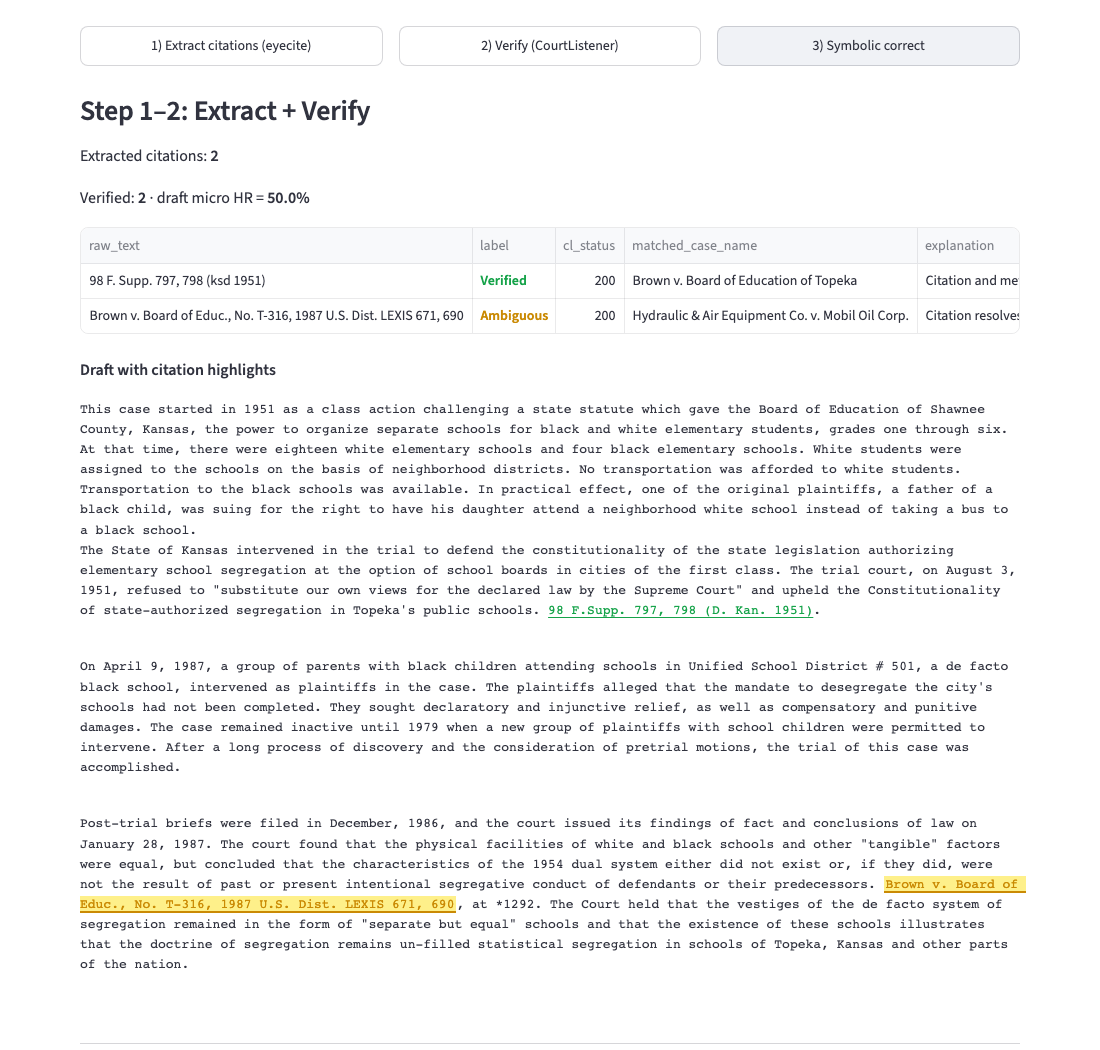
\includegraphics[width=0.92\linewidth]{live_pipeline_extract_verify.png}
\caption{Live pipeline demonstration on case \texttt{SD-KS-0001}, extraction and verification: eyecite finds 2 citations; CourtListener labels one Verified and one Ambiguous (draft paired HR 50\%), and the draft text is highlighted accordingly.}
\label{fig:live-pipeline-extract-verify}
\end{figure}

\begin{figure}[!t]
\centering
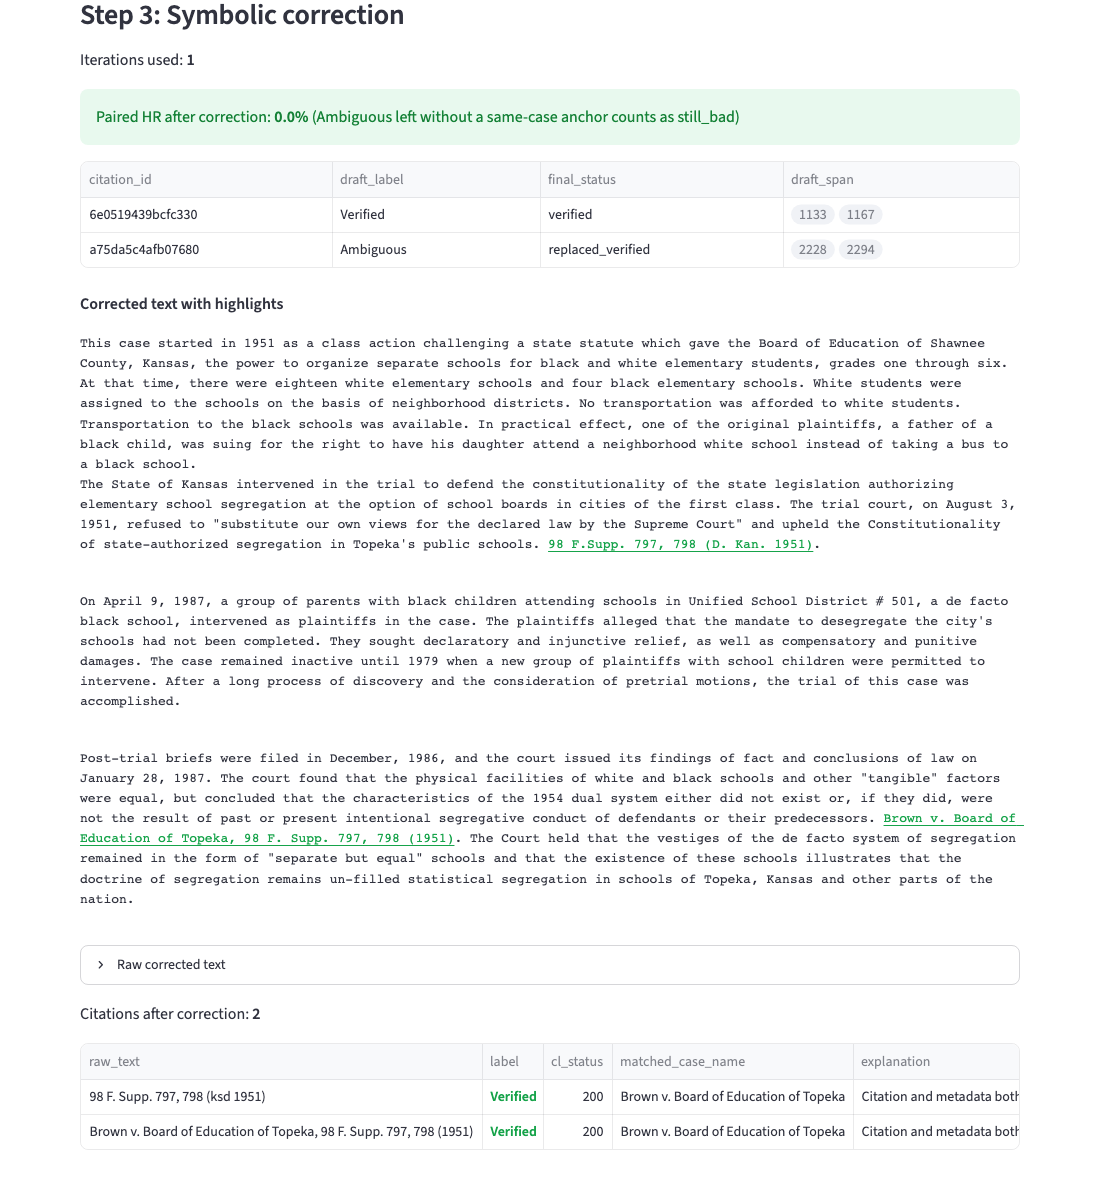
\includegraphics[width=0.92\linewidth]{live_pipeline_correction.png}
\caption{Live pipeline demonstration on case \texttt{SD-KS-0001}, symbolic correction: the Ambiguous LEXIS citation is re-anchored to the Verified reporter citation already present in the same summary, taking paired HR to 0\% after 1 correction iteration.}
\label{fig:live-pipeline-correction}
\end{figure}

\subsection{Why a rented GPU instance, and its measured cost}
\label{sec:method-compute-cost}

Two of the three generators, and the single full-scale PRIMERA run, needed sustained, uninterrupted GPU access: PRIMERA's 100-case $D\rightarrow L$ batch and the two Qwen2.5-7B-Instruct conditions each ran as one continuous generation pass over the identical case set, checkpointing after every case but never pausing for a multi-hour wait. Google Colab's free tier caps continuous session length and disconnects without warning, which risks losing an in-progress batch partway through and re-generating cases already produced. A rented on-demand GPU instance (RunPod, one NVIDIA RTX~4090 per session) removed that risk for the only GPU-bound phase of the pipeline. CourtListener verification, extraction, and correction (Sections~\ref{sec:module-b}--\ref{sec:correction}) run locally afterward and do not need a GPU; renting compute only for generation, rather than for the multi-day CourtListener-rate-limited wait that follows (Section~\ref{sec:module-c}), kept the pod running only while it was doing GPU work.

Table~\ref{tab:runpod-cost} reports the measured GPU time for each generation run, read directly from the pipeline's own per-run completion logs, and its cost at the rented instance's \$0.49/hour rate.

\begin{table}[!t]
\centering
\caption{RunPod RTX~4090 generation cost by condition (measured GPU time, \$0.49/hour).}
\label{tab:runpod-cost}
\begin{tabular}{@{}l r r@{}}
\toprule
\textbf{Generator} & \textbf{GPU time} & \textbf{Cost} \\
\midrule
PRIMERA (baseline) & 10.3 min (0.17 h) & \$0.08 \\
LLM zero-shot & 57.4 min (0.96 h) & \$0.47 \\
LLM + retrieval & 59.0 min (0.98 h) & \$0.48 \\
\midrule
\textbf{Total} & \textbf{126.7 min (2.11 h)} & \textbf{\$1.03} \\
\bottomrule
\end{tabular}
\end{table}

This figure covers measured generation compute only; it excludes the smaller, untimed overhead of environment setup, dependency installation, and pre-generation checks that ran once per pod session before generation started. The full-scale run's only GPU-bound phase, across all three generators, cost on the order of one U.S. dollar.

\section{Ethics, Limits, and Design Honesty}
\label{sec:method-ethics}

Multi-LexSum summaries are CC~BY-NC; raw text used for internal audit remains coursework-restricted. CourtListener lookups are rate-limited public API calls. The methodology does not claim that re-anchoring recovers the historically perfect reporter citation for every Ambiguous span, only that it is safer than inserting a contradicting case name. Truncation, OCR noise, and proprietary identifier fragility remain acknowledged threats to both generation and verification.

\section{Chapter Summary}
\label{sec:method-summary}

Methodology operationalizes the thesis story: EDA motivated $D\rightarrow L$ and untrusted drafts; Modules~A--C implement generate--extract--verify; correction privileges auditability over aggressive rewriting; paired HR measures whether draft hallucinations survive. The next chapter outlines the formal evaluation protocol under which these components are scored.
